\documentclass[a4paper,14pt]{extarticle}

\usepackage[utf8x]{inputenc}
\usepackage[T1]{fontenc}
\usepackage[russian]{babel}
\usepackage{hyperref}
\usepackage{indentfirst}
\usepackage{here}
\usepackage{array}
\usepackage{graphicx}
\usepackage{caption}
\usepackage{subcaption}
\usepackage{chngcntr}
\usepackage{amsmath}
\usepackage{amssymb}
\usepackage[left=2cm,right=2cm,top=2cm,bottom=2cm,bindingoffset=0cm]{geometry}
\usepackage{multicol}
\usepackage{multirow}
\usepackage{titlesec}
\usepackage{listings}
\usepackage{color}
\usepackage{enumitem}
\usepackage{cmap}
\usepackage{listingsutf8}

\definecolor{green}{rgb}{0,0.6,0}
\definecolor{gray}{rgb}{0.5,0.5,0.5}
\definecolor{purple}{rgb}{0.58,0,0.82}

\lstdefinelanguage{none}{}

\lstset{
	language={SQL},
	inputpath={../sql/},
	backgroundcolor=\color{white},
	commentstyle=\color{green},
	keywordstyle=\color{blue},
	numberstyle=\color{gray}\scriptsize\ttfamily,
	stringstyle=\color{purple},
	basicstyle=\lst@ifdisplaystyle\footnotesize\fi\ttfamily,
	breakatwhitespace=false,
	breaklines=true,
	captionpos=b,
	keepspaces=true,
	numbers=left,
	numbersep=5pt,
	showspaces=false,
	showstringspaces=false,
	showtabs=false,
	tabsize=4,
	frame=single,
	morekeywords={IF, BIGSERIAL, SERIAL, TEXT, BIGINT, MONEY, BOOLEAN, REFERENCES},
	deletekeywords={count, error},
	morecomment=[l][\color{green}]{\$\$},
	sensitive=true,
	columns=fullflexible,
	inputencoding=utf8/cp1251
}

\renewcommand{\le}{\ensuremath{\leqslant}}
\renewcommand{\leq}{\ensuremath{\leqslant}}
\renewcommand{\ge}{\ensuremath{\geqslant}}
\renewcommand{\geq}{\ensuremath{\geqslant}}
\renewcommand{\epsilon}{\ensuremath{\varepsilon}}
\renewcommand{\phi}{\ensuremath{\varphi}}
\renewcommand{\thefigure}{\arabic{figure}}
\newcommand{\code}[1]{\lstinline|#1|}
\newcommand{\caret}{\^{}}

\titleformat*{\section}{\large\bfseries} 
\titleformat*{\subsection}{\normalsize\bfseries} 
\titleformat*{\subsubsection}{\normalsize\bfseries} 
\titleformat*{\paragraph}{\normalsize\bfseries} 
\titleformat*{\subparagraph}{\normalsize\bfseries} 

\counterwithin{figure}{section}
\counterwithin{equation}{section}
\counterwithin{table}{section}
\newcommand{\sign}[1][5cm]{\makebox[#1]{\hrulefill}}
\newcommand{\equipollence}{\quad\Leftrightarrow\quad}
\newcommand{\no}[1]{\overline{#1}}
\graphicspath{{../../migrations/}}
\captionsetup{justification=centering,margin=1cm}
\def\arraystretch{1.3}
\setlength\parindent{5ex}
\titlelabel{\thetitle.\quad}

\setitemize{topsep=0em, itemsep=0em}
\setenumerate{topsep=0em, itemsep=0em}

\begin{document}

\begin{titlepage}	% начало титульной страницы

	\begin{center}		% выравнивание по центру

		\large Санкт-Петербургский Политехнический Университет Петра Великого\\
		\large Институт компьютерных наук и технологий \\
		\large Кафедра компьютерных систем и программных технологий\\[6cm]
		% название института, затем отступ 6см
		
		\huge Базы данных\\[0.5cm] % название работы, затем отступ 0,5см
		\large Отчет по лабораторной работе №1\\[0.1cm]
		\large Проектирование модели БД\\[5cm]

	\end{center}


	\begin{flushright} % выравнивание по правому краю
		\begin{minipage}{0.25\textwidth} % врезка в половину ширины текста
			\begin{flushleft} % выровнять её содержимое по левому краю

				\large\textbf{Работу выполнил:}\\
				\large Курякин Д. А.\\
				\large {Группа:} 43501/3\\
				
				\large \textbf{Преподаватель:}\\
				\large Мяснов А.В.

			\end{flushleft}
		\end{minipage}
	\end{flushright}
	
	\vfill % заполнить всё доступное ниже пространство

	\begin{center}
	\large Санкт-Петербург\\
	\large \the\year % вывести дату
	\end{center} % закончить выравнивание по центру

\thispagestyle{empty} % не нумеровать страницу
\end{titlepage} % конец титульной страницы

\vfill % заполнить всё доступное ниже пространство


\tableofcontents
\newpage

\section{Цель работы}

Познакомиться с основами проектирования схемы БД, языком описания сущностей и ограничений БД SQL-DDL.

\section{Программа работы}

\begin{enumerate}
	\item Самостоятельное изучение SQL-DDL.
	\item Создание скрипта БД в соответствии с согласованной схемой. Должны присутствовать первичные и внешние ключи, ограничения на диапазоны значений. Демонстрация скрипта преподавателю. 
	\item Создание скрипта, заполняющего все таблицы БД данными.
	\item Выполнение SQL-запросов, изменяющих схему созданной БД по заданию преподавателя. Демонстрация их работы преподавателю.
\end{enumerate}

\section{Теоретическая информация}

\textbf{Язык SQL} (Structured Query Language) -- язык структурированных запросов. Он позволяет формировать весьма сложные запросы к базам данных. В SQL определены два подмножества языка:

\begin{itemize}
	\item \textbf{SQL-DDL} (Data Definition Language) -- язык определения структур и ограничений целостности баз данных. Сюда относятся команды создания и удаления баз данных; создания, изменения и удаления таблиц; управления пользователями и т.д.
	\item \textbf{SQL-DML} (Data Manipulation Language) -- язык манипулирования данными: добавление, изменение, удаление и извлечение данных, управления транзакциями. Функции SQL-DML определяются первым словом в предложении (часто называемом запросом), которое является глаголом: \code{SELECT} (<<выбрать>>), \code{INSERT} (<<вставить>>), \code{UPDATE} (<<обновить>>), и \code{DELETE} (<<удалить>>). 
\end{itemize}

\section{Выполнение работы}

\subsection{Структура базы данных}

\begin{figure}[H]
	\begin{center}
		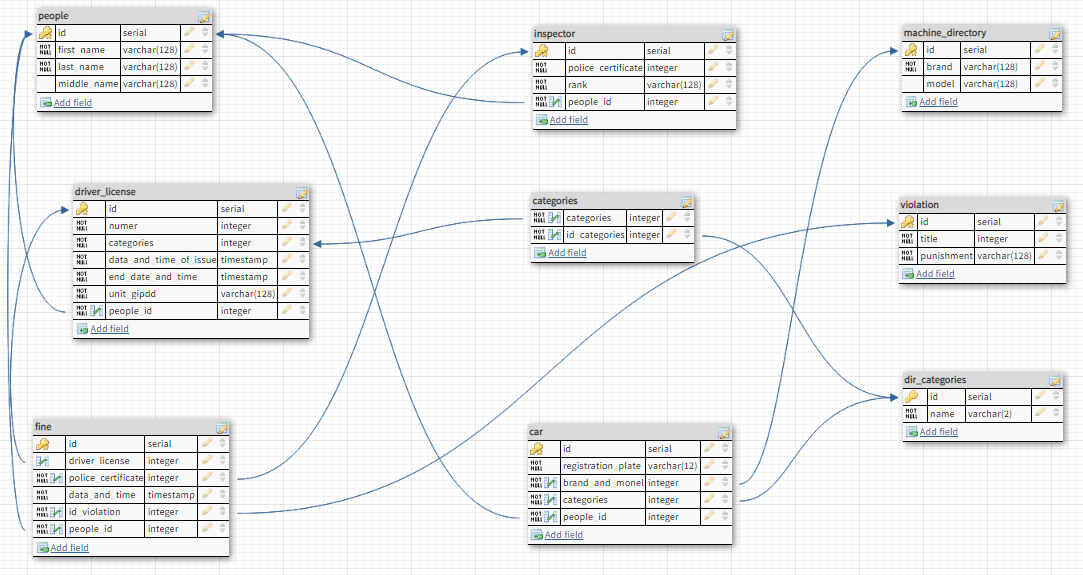
\includegraphics[scale=0.6]{../../diagram/diagram.png}
		\caption{Схема модели} 
		\label{pic:pic_name} % название для ссылок внутри кода
	\end{center}
\end{figure}

\subsection{Скрипт создания структуры базы данных}

\lstinputlisting{../sql/table.sql}

\subsection{Скрипт заполнения таблиц тестовыми данными}

\lstinputlisting{../sql/filling.sql}

После внесения дополнительных требований преподавателя была изменена структура базы данных, добавленны таблицы и добавленны тестовые данные.

\subsection{Структура базы данных после изменения}

\begin{figure}[H]
	\begin{center}
		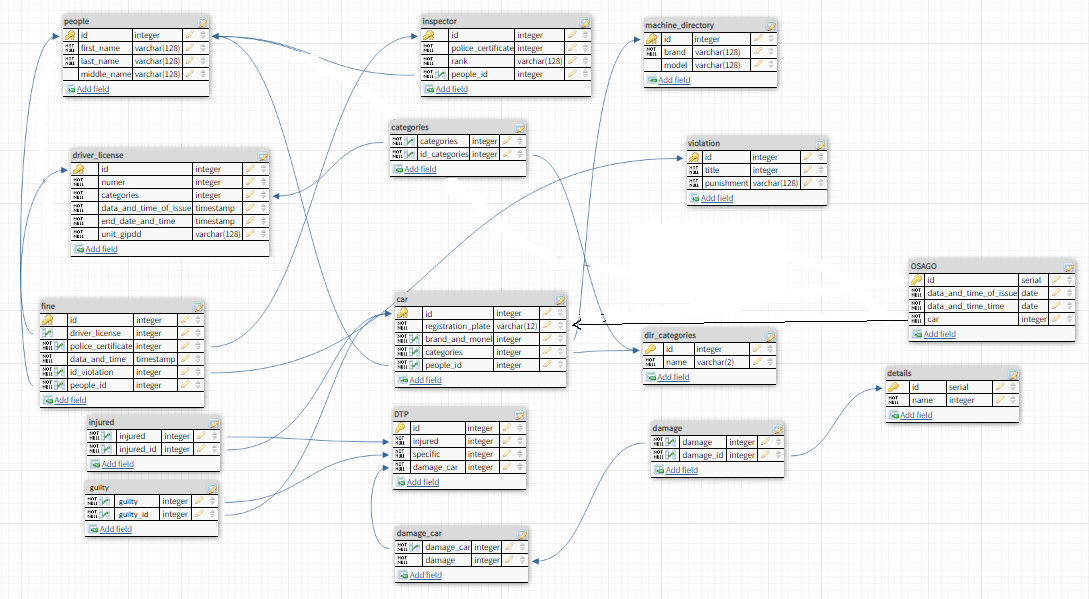
\includegraphics[scale=0.6]{../../diagram/diagram2.png}
		\caption{Схема модели 2} 
		\label{pic:pic_name2} % название для ссылок внутри кода
	\end{center}
\end{figure}

\subsection{Скрипт создания структуры базы данных после изменения}

\lstinputlisting{../sql/table2.sql}

\subsection{Скрипт заполнения таблиц тестовыми данными после изменения}

\lstinputlisting{../sql/filling2.sql}

Во время выполнения 3 лабораторной работы в качастве первичных лю
При выполнение 3 лабораторной работы первичные ключи были типа Integer. В последствие типы первичных лючей были изменены а serial.

\subsection{Скрипт создания структуры базы данны первичный ключ serial}

\lstinputlisting{../sql/table3.sql}

\subsection{Скрипт заполнения таблиц тестовыми данными первичный ключ seria}

\lstinputlisting{../sql/filling3.sql}

\section{Выводы}

В ходе выполнения данной работы были изучены основы создания скриптов на языке SQL. С помощью SQL-DDL описаны структуры разрабатываемой схемы базы данных. С использованием SQL-DML созданные структуры заполнены тестовыми данными. Изучен синтаксис обновления структуры существующей таблицы.

\end{document}
